\documentclass{standalone}
\usepackage{tikz}
\usetikzlibrary{patterns, positioning}
\usepackage[sfdefault]{ClearSans} %% option 'sfdefault' activates Clear Sans as the default text font
\usepackage[T1]{fontenc}

\begin{document}
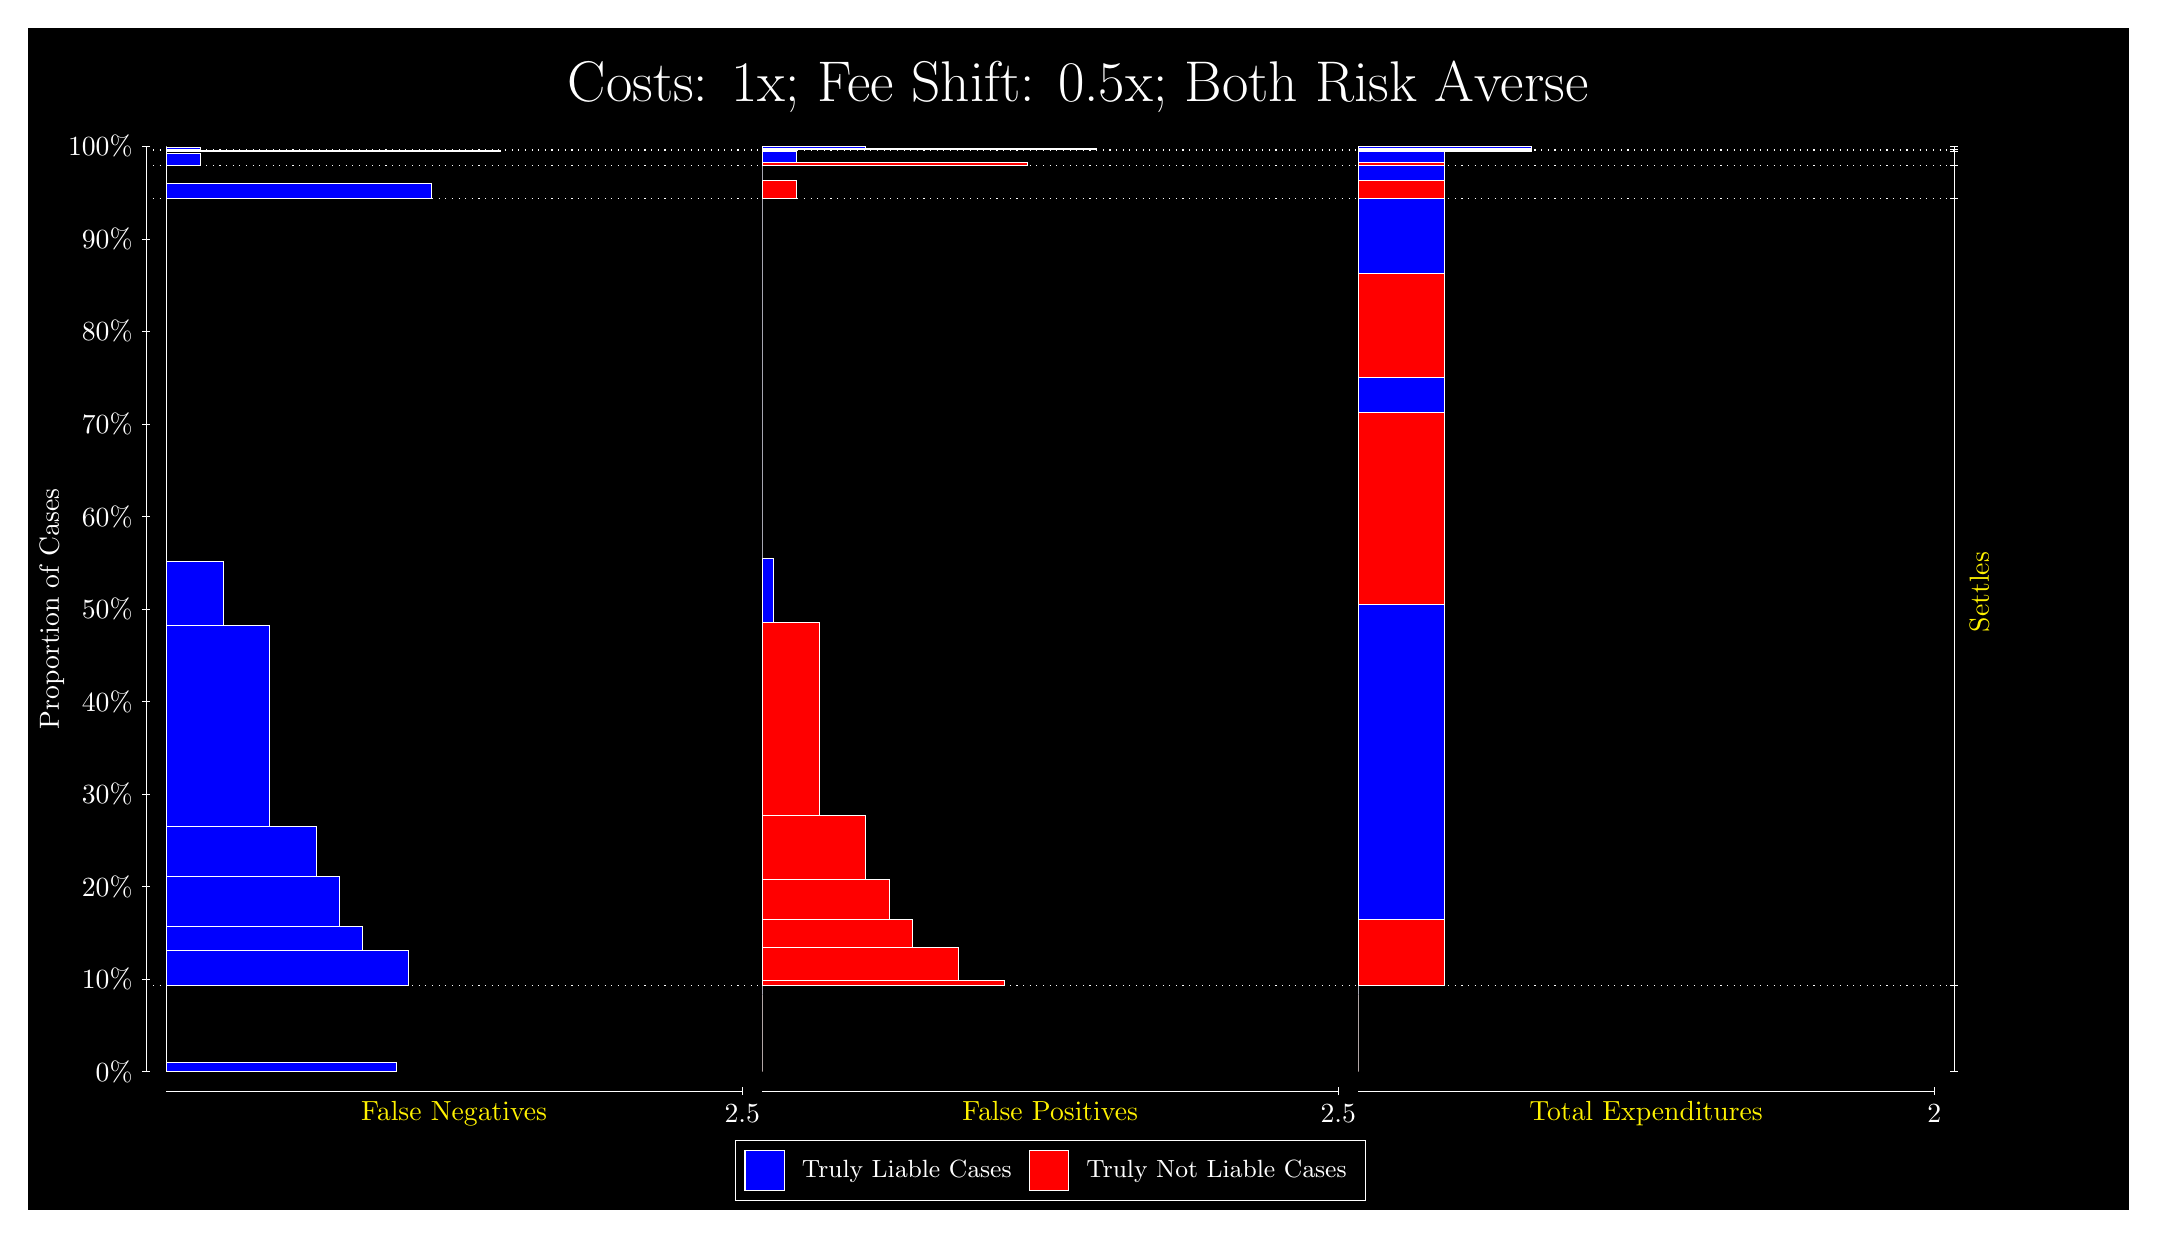
\begin{tikzpicture}
\draw[fill=black] (0,0) rectangle (26.667,15);
\draw[text=white] (0,13.5) rectangle (26.667,15) node[midway] {\huge Costs: 1x; Fee Shift: 0.5x; Both Risk Averse};
\draw[white, very thin] (1.5,1.75) -- (1.5,13.5);
\node[rotate=90, text=white, anchor=center] at (0.3, 7.625) {Proportion of Cases};
\draw[white, very thin] (1.45,1.75) -- (1.55,1.75);
\node[text=white, anchor=east] at (1.45, 1.75) {0\%};
\draw[white, very thin] (1.45,2.925) -- (1.55,2.925);
\node[text=white, anchor=east] at (1.45, 2.925) {10\%};
\draw[white, very thin] (1.45,4.1) -- (1.55,4.1);
\node[text=white, anchor=east] at (1.45, 4.1) {20\%};
\draw[white, very thin] (1.45,5.275) -- (1.55,5.275);
\node[text=white, anchor=east] at (1.45, 5.275) {30\%};
\draw[white, very thin] (1.45,6.45) -- (1.55,6.45);
\node[text=white, anchor=east] at (1.45, 6.45) {40\%};
\draw[white, very thin] (1.45,7.625) -- (1.55,7.625);
\node[text=white, anchor=east] at (1.45, 7.625) {50\%};
\draw[white, very thin] (1.45,8.8) -- (1.55,8.8);
\node[text=white, anchor=east] at (1.45, 8.8) {60\%};
\draw[white, very thin] (1.45,9.975) -- (1.55,9.975);
\node[text=white, anchor=east] at (1.45, 9.975) {70\%};
\draw[white, very thin] (1.45,11.15) -- (1.55,11.15);
\node[text=white, anchor=east] at (1.45, 11.15) {80\%};
\draw[white, very thin] (1.45,12.325) -- (1.55,12.325);
\node[text=white, anchor=east] at (1.45, 12.325) {90\%};
\draw[white, very thin] (1.45,13.5) -- (1.55,13.5);
\node[text=white, anchor=east] at (1.45, 13.5) {100\%};

\draw[white, very thin] (24.457,1.75) -- (24.457,13.5);
\draw[white, very thin] (24.407,1.75) -- (24.507,1.75);
\node[anchor=west] at (24.407, 1.75) {};
\draw[white, very thin] (24.407,2.8432) -- (24.507,2.8432);
\node[anchor=west] at (24.407, 2.8432) {};
\draw[white, very thin] (24.407,12.837) -- (24.507,12.837);
\node[anchor=west] at (24.407, 12.837) {};
\draw[white, very thin] (24.407,13.26) -- (24.507,13.26);
\node[anchor=west] at (24.407, 13.26) {};
\draw[white, very thin] (24.407,13.443) -- (24.507,13.443);
\node[anchor=west] at (24.407, 13.443) {};
\draw[white, very thin] (24.407,13.462) -- (24.507,13.462);
\node[anchor=west] at (24.407, 13.462) {};
\draw[white, very thin] (24.407,13.5) -- (24.507,13.5);
\node[anchor=west] at (24.407, 13.5) {};

\draw[white, very thin, fill=blue] (1.75,1.75) rectangle (4.6775,1.865);
\draw[white, very thin, fill=red] (1.75,1.865) rectangle (1.75,2.8432);
\draw[white, very thin, fill=blue] (1.75,2.8432) rectangle (4.8239,3.2841);
\draw[white, very thin, fill=blue] (1.75,3.2841) rectangle (4.2384,3.6007);
\draw[white, very thin, fill=blue] (1.75,3.6007) rectangle (3.9457,4.236);
\draw[white, very thin, fill=blue] (1.75,4.236) rectangle (3.6529,4.8586);
\draw[white, very thin, fill=blue] (1.75,4.8586) rectangle (3.0674,7.4157);
\draw[white, very thin, fill=blue] (1.75,7.4157) rectangle (2.4819,8.224);
\draw[white, very thin, fill=red] (1.75,8.224) rectangle (1.75,12.837);
\draw[white, very thin, fill=blue] (1.75,12.837) rectangle (5.1167,13.029);
\draw[white, very thin, fill=red] (1.75,13.029) rectangle (1.75,13.26);
\draw[white, very thin, fill=blue] (1.75,13.26) rectangle (2.1891,13.409);
\draw[white, very thin, fill=red] (1.75,13.409) rectangle (1.75,13.443);
\draw[white, very thin, fill=blue] (1.75,13.443) rectangle (5.9949,13.453);
\draw[white, very thin, fill=red] (1.75,13.453) rectangle (1.75,13.462);
\draw[white, very thin, fill=blue] (1.75,13.462) rectangle (2.1891,13.491);
\draw[white, very thin, fill=red] (1.75,13.491) rectangle (1.75,13.5);
\draw[white, very thin, fill=red] (9.3189,1.75) rectangle (9.3189,2.7282);
\draw[white, very thin, fill=blue] (9.3189,2.7282) rectangle (9.3189,2.8432);
\draw[white, very thin, fill=red] (9.3189,2.8432) rectangle (12.393,2.9122);
\draw[white, very thin, fill=red] (9.3189,2.9122) rectangle (11.807,3.3269);
\draw[white, very thin, fill=red] (9.3189,3.3269) rectangle (11.222,3.6898);
\draw[white, very thin, fill=red] (9.3189,3.6898) rectangle (10.929,4.1905);
\draw[white, very thin, fill=red] (9.3189,4.1905) rectangle (10.636,5.0078);
\draw[white, very thin, fill=red] (9.3189,5.0078) rectangle (10.051,7.4561);
\draw[white, very thin, fill=blue] (9.3189,7.4561) rectangle (9.4652,8.2644);
\draw[white, very thin, fill=blue] (9.3189,8.2644) rectangle (9.3189,12.837);
\draw[white, very thin, fill=red] (9.3189,12.837) rectangle (9.758,13.068);
\draw[white, very thin, fill=blue] (9.3189,13.068) rectangle (9.3189,13.26);
\draw[white, very thin, fill=red] (9.3189,13.26) rectangle (12.686,13.294);
\draw[white, very thin, fill=blue] (9.3189,13.294) rectangle (9.758,13.443);
\draw[white, very thin, fill=red] (9.3189,13.443) rectangle (9.758,13.453);
\draw[white, very thin, fill=blue] (9.3189,13.453) rectangle (9.3189,13.462);
\draw[white, very thin, fill=red] (9.3189,13.462) rectangle (13.564,13.471);
\draw[white, very thin, fill=blue] (9.3189,13.471) rectangle (10.636,13.5);
\draw[white, very thin, fill=red] (16.888,1.75) rectangle (16.888,2.7282);
\draw[white, very thin, fill=blue] (16.888,2.7282) rectangle (16.888,2.8432);
\draw[white, very thin, fill=red] (16.888,2.8432) rectangle (17.986,3.6898);
\draw[white, very thin, fill=blue] (16.888,3.6898) rectangle (17.986,7.6778);
\draw[white, very thin, fill=red] (16.888,7.6778) rectangle (17.986,10.126);
\draw[white, very thin, fill=blue] (16.888,10.126) rectangle (17.986,10.567);
\draw[white, very thin, fill=red] (16.888,10.567) rectangle (17.986,11.885);
\draw[white, very thin, fill=blue] (16.888,11.885) rectangle (17.986,12.837);
\draw[white, very thin, fill=red] (16.888,12.837) rectangle (17.986,13.068);
\draw[white, very thin, fill=blue] (16.888,13.068) rectangle (17.986,13.26);
\draw[white, very thin, fill=red] (16.888,13.26) rectangle (17.986,13.294);
\draw[white, very thin, fill=blue] (16.888,13.294) rectangle (17.986,13.443);
\draw[white, very thin, fill=red] (16.888,13.443) rectangle (19.083,13.453);
\draw[white, very thin, fill=blue] (16.888,13.453) rectangle (19.083,13.462);
\draw[white, very thin, fill=red] (16.888,13.462) rectangle (19.083,13.471);
\draw[white, very thin, fill=blue] (16.888,13.471) rectangle (19.083,13.5);
\draw[white, dotted] (1.5,2.8432) -- (24.457,2.8432);
\draw[white, dotted] (1.5,12.837) -- (24.457,12.837);
\draw[white, dotted] (1.5,13.26) -- (24.457,13.26);
\draw[white, dotted] (1.5,13.443) -- (24.457,13.443);
\draw[white, dotted] (1.5,13.462) -- (24.457,13.462);
\draw[white, very thin] (1.75,1.5) -- (9.0689,1.5);
\node[text=yellow, anchor=north] at (5.4094, 1.5) {False Negatives};
\draw[white, very thin] (9.0689,1.45) -- (9.0689,1.55);
\node[text=white, anchor=north] at (9.0689, 1.45) {2.5};

\draw[white, very thin] (9.3189,1.5) -- (16.638,1.5);
\node[text=yellow, anchor=north] at (12.978, 1.5) {False Positives};
\draw[white, very thin] (16.638,1.45) -- (16.638,1.55);
\node[text=white, anchor=north] at (16.638, 1.45) {2.5};

\draw[white, very thin] (16.888,1.5) -- (24.207,1.5);
\node[text=yellow, anchor=north] at (20.547, 1.5) {Total Expenditures};
\draw[white, very thin] (24.207,1.45) -- (24.207,1.55);
\node[text=white, anchor=north] at (24.207, 1.45) {2};


\node[text=yellow, centered, rotate=90] at (24.777, 7.84) {Settles};





\draw (12.978300999999998,1.5) node[draw=none] (baseCoordinate) {};
\begin{scope}[align=center]
        \matrix[scale=0.5, draw=white, below=0.5cm of baseCoordinate, nodes={draw}, column sep=0.1cm]{
            \node[rectangle, draw, minimum width=0.5cm, minimum height=0.5cm, fill=blue] {}; &
            \node[draw=none, font=\small, text=white] (B) {Truly Liable Cases}; &
            \node[rectangle, draw, minimum width=0.5cm, minimum height=0.5cm, fill=red] {}; &
            \node[draw=none, font=\small, text=white] (B) {Truly Not Liable Cases}; \\
            };
\end{scope}

\end{tikzpicture}
\end{document}